% slide 1: wiki and overlinking
% slide 2: the figure 1 - converting to ranking problem
% slide 3: the 3 questions

\begin{frame}
  \frametitle{Wikipedia}  
\begin{columns}
  \begin{column}{0.5\textwidth}
    \begin{itemize}
      \item Internet Encyclopedia
      \item Wikimedia Foundation
      \item Free-Content
      \item Free-of-Cost
      \item 38 million articles
      \item 250 languages
      \item 500 million unique visitors per month
  \end{itemize}
\end{column}
\begin{column}{0.5\textwidth}  %%<--- here
    \begin{center}
     
\includegraphics[width=0.5\textwidth]{images/Wikipedia-logo-en-big.png}
     \end{center}
\end{column}
\end{columns}

\end{frame}



\begin{frame}
  \frametitle{Overlinking}
  
  \centering \textit{"In the English Wikipedia, of all the 800,000 links added to the site in February 2015, the majority (66~\%) were not clicked even a single time in March"}
  
  %\begin{figure}[tbph]
  %  \centering
  %  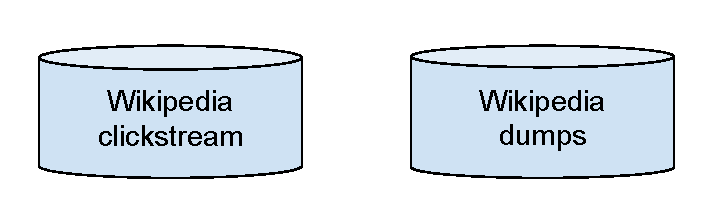
\includegraphics[width=0.7\linewidth]{images/datasets}
  %\end{figure}
  
\end{frame}

\begin{frame}
  \frametitle{Ranking Problem}
  Transforming Overlinking problem to Ranking Problem.
  \begin{figure}[tbph]
    \centering
    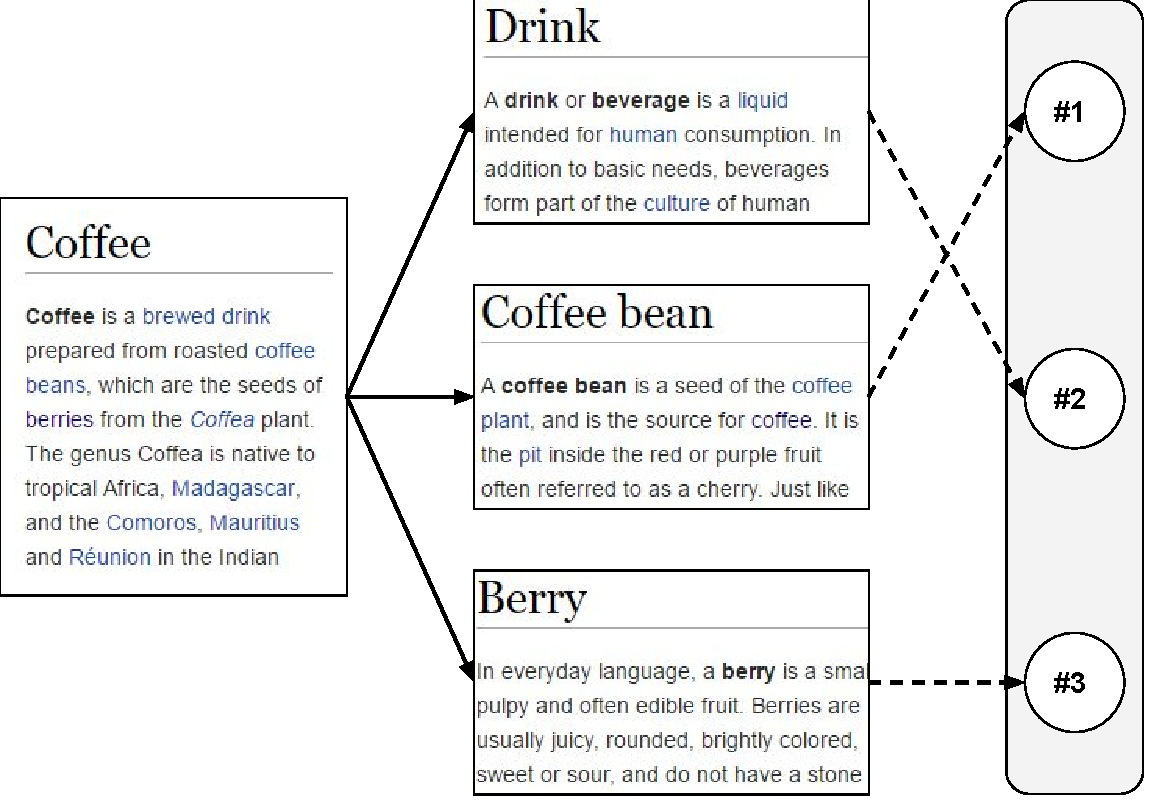
\includegraphics[width=0.7\linewidth]{images/concept}
  \end{figure}
  
\end{frame}

\begin{frame}
  \frametitle{Research Questions}
  \begin{enumerate}
	\item Which features of the articles influence the click frequency of links the most?
	\item To what extent can we use the Learning to Rank algorithm to predict relevance of links?
	\item Can Learning to Rank help with reducing overlinking problem?
  \end{enumerate}
\end{frame}

